\begin{figure}
	\centering
	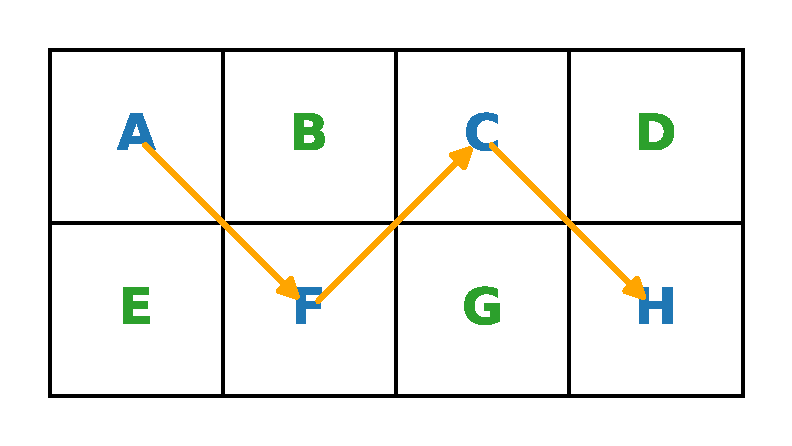
\includegraphics[width=\textwidth]{Diagrams/ZigZag/ZigZag.pdf}
	\caption{Three quadratic Bezier curves with C0 continuity stored in a 4x2 texture, instead of an 8x2 texture. The orange line shows how to sample the texture as t varies in $[0,3]$.
    The average of the green pixels opposite the orange lines define the middle control point. For $N$ curves, there will always be $N$ constraints with $N+1$ free variables to satisfy them.}
	\label{fig_ZigZag}
\end{figure}
